\subsection{MOLGEN}
{{\footnotesize
\noindent MolGen is a pre-trained molecular language model that generates chemically valid
molecules using SELFIES and reinforcement learning, guided by chemical feedback 
to optimize properties such as logP, QED, and docking score.


\begin{description}[labelwidth=4cm, labelsep=1em, leftmargin=4cm, itemsep=0.1em, parsep=0em]
  \item[date:] 2023-01-26
  \item[version:] 1
  \item[last\_updated:] 2023-01-26
  \item[expired:] false
  \item[valid:] yes
  \item[valid\_date:] 2023-01-26
  \item[url:] \href{https://github.com/zjunlp/MolGen}{https://github.com/zjunlp/MolGen}
  \item[doi:] 10.48550/arXiv.2301.11259
  \item[domain:] Computational Chemistry
  \item[focus:] Molecular generation and optimization
  \item[keywords:]
    - SELFIES
    - GAN
    - property optimization
  \item[licensing:] MIT License
  \item[task\_types:]
    - Distribution learning
    - Goal-oriented generation
  \item[ai\_capability\_measured:]
    - Generation of valid and optimized molecular structures
  \item[metrics:]
    - Validity\%
    - Novelty\%
    - QED
    - Docking score
  \item[models:]
    - MolGen
  \item[ml\_motif:]
    - Chemical generation
  \item[type:] Benchmark
  \item[ml\_task:]
    - Supervised Learning
  \item[solutions:] 0
  \item[notes:] This is a model, not a benchmark
  \item[contact.name:] unknown
  \item[contact.email:] unknown
  \item[datasets.links.name:] unknown
  \item[datasets.links.url:] \href{unknown}{unknown}
  \item[results.links.name:] unknown
  \item[results.links.url:] \href{unknown}{unknown}
  \item[fair.reproducible:] True
  \item[fair.benchmark\_ready:] True
  \item[id:] molgen
  \item[Citations:] \cite{fang2024domainagnosticmoleculargenerationchemical}
\end{description}

{\bf Ratings:} ~ \\

\begin{tabular}{p{0.15\textwidth} p{0.07\textwidth} p{0.7\textwidth}}
\hline
Rating & Value & Reason \\
\hline
dataset & 0 & This is a pre-trained model
 \\
documentation & 0 & This is a pre-trained model
 \\
metrics & 0 & This is a pre-trained model
 \\
reference\_solution & 0 & This is a pre-trained model
 \\
software & 0 & This is a pre-trained model
 \\
specification & 0 & This is a pre-trained model
 \\
\hline
\end{tabular}

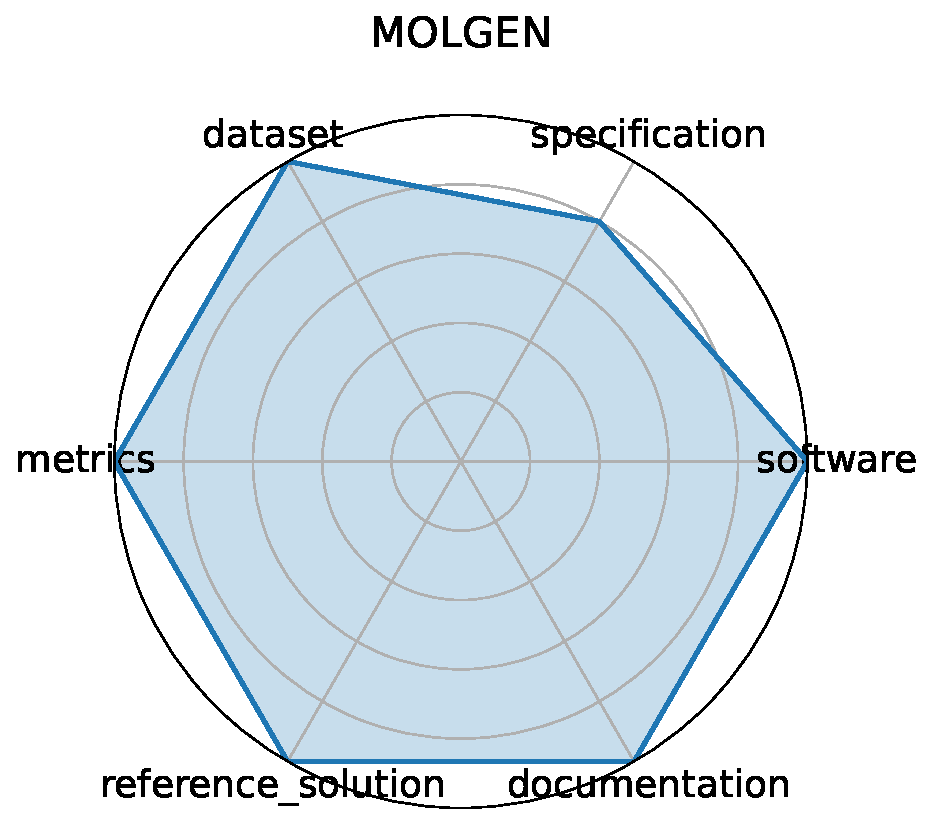
\includegraphics[width=0.2\textwidth]{molgen_radar.pdf}
}}
\clearpage